\documentclass[a4paper,14pt]{article}
\usepackage[utf8]{inputenc}
\usepackage[T1]{fontenc}
\usepackage{mathptmx}
\usepackage{geometry}
\usepackage{mathtools}
\usepackage[english]{babel}
\usepackage{graphicx}
\usepackage{subcaption}
\usepackage[figurename=Figure]{caption}
\usepackage{hyperref}
\usepackage{minted}
\usepackage{setspace}
\usepackage{color}
\usepackage[explicit]{titlesec}
\usepackage{tocloft}
\usepackage{titletoc}
\usepackage{indentfirst}
\usepackage{caption}
\usepackage{subcaption}
\usepackage{amsmath} 
\usepackage{pdfpages}

\hypersetup{colorlinks,
	citecolor=black,
	filecolor=black,
	linkcolor=black,
	urlcolor=black
}

\geometry{
	a4paper,
	left=20mm,
	right=15mm,
	top=10mm,
	bottom=10mm,
}

\date{}

%=============================================================================
% Modified Items

\titleformat{\section}{}{}{14pt}{\textbf{References:}}
\pagenumbering{gobble}

%=============================================================================

\begin{document}

% untuk judul
\begin{center}
	\textbf{Experimental Study of Multi-Point Intrusion Detector Based On Optical Time Domain Reflectometry}
\end{center}

% untuk author
\begin{center}
	Agus Muhammad Hatta, Achmadi \\
	Engineering Physics, Institut Teknologi Sepuluh Nopember, Indonesia
\end{center}

% untuk penanda
\begin{center}
	\textit{Extended Abstract}
\end{center}

Intrusion by an intruder is an act that cannot be ignored due to a building, an area (perimeter), or any object regarding it’s either military, economical, or industrial values.
Intrusion has high similarity to thieft crime and can be root of more crime act.
Intrusion is an act that by-passing any survelleince or security system.
For prevention, a detection system become essential to many security system.
This detection system has to be highly accurate and fast respons.
Optical fiber already known for it’s capabilities to both data transmission and as a distributed sensor.
An distributed sensor mean single optical fiber section can replace many point-type sensors.
The OTDR system already known as one of optical fiber characterization.
There is many commercial brand for intrusion detector system based on optical fiber and OTDR.
However most of those brand require special OTDR, like phase-sensitive OTDR or frequency-based reflectometry, instead an ordinary OTDR.
This leads to developement of a intrusion detection system that limit the design only on optical fiber sensor setup instead modify the OTDR instrument.
As a start, this research provide characteristic summary for some optical-fiber sensor setup and propose best result to implement as intruder detector system.

\hfill

This paper presents result comparisson of some various optical-fiber sensor setup that combination of single-mode, graded-index multi-mode, and step-index multi-mode optical-fiber.
In order to get intrusion input, a measured single displacement applied to these sensor setup.\cite{Pinto2006}.
To apply displacement, optical-fiber installed on iron string with length (as \textbf{L}) 1m and 5m.
Then a fix displacement applied to iron string with distance (as \textbf{d}) 5mm, 10mm, 15mm, 20mm, and 25mm.  
All test using only wave length 1550nm with 20ns pulse-width using Anritsu MU909015C OTDR instrument.\cite{Anritsu2010} 

\begin{figure}[h!]
	\centering
	\captionsetup{justification=centering}
	\includegraphics[width=0.6\linewidth]{images/setup}
	\caption[Setup Diagram]{\small{Test setup diagram}}
\end{figure}

All trace result recorded on OTDR instrument for each length and distance.
Only fiber-splice and fiber-end that taken to analysis instead all trace data-point.
For each event, the maximum value are compared to initial (no-input) condition.

\begin{figure}[h!]
	\centering
	\captionsetup{justification=centering}
	\begin{subfigure}[b]{0.4\textwidth}
		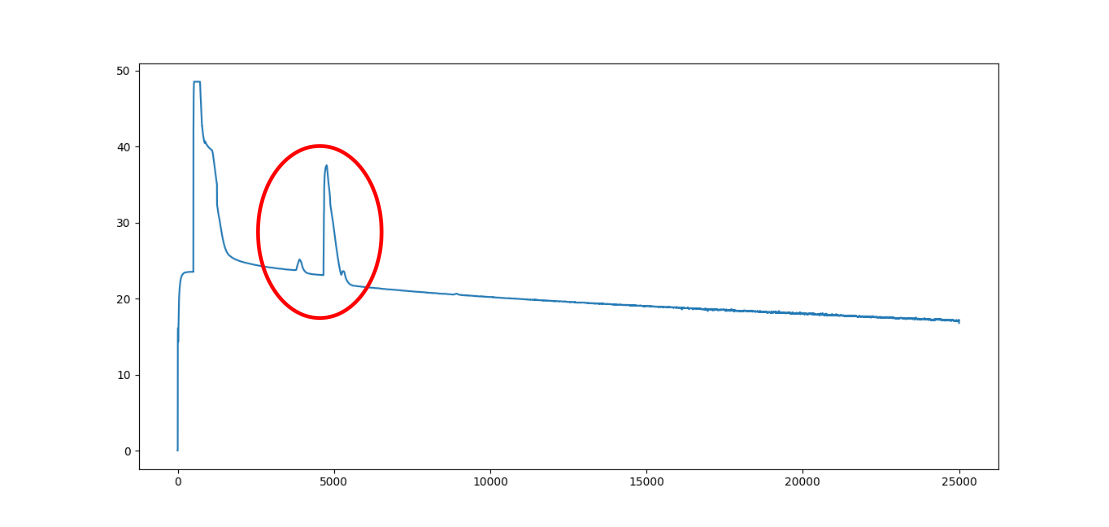
\includegraphics[width=\textwidth]{images/base}
		\caption{}
	\end{subfigure}
	\begin{subfigure}[b]{0.4\textwidth}
		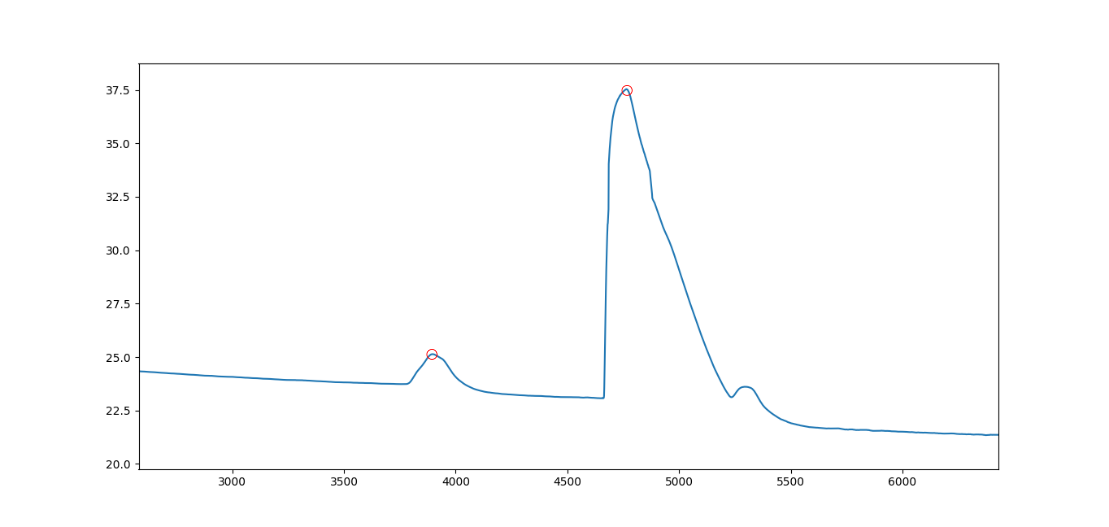
\includegraphics[width=\textwidth]{images/take_point}
		\caption{}
	\end{subfigure}
	\caption[Setup Diagram]{\small{(a) Trace result part to be analyzed. (b) First peak is fiber-splice event and second peak is fiber-end event}}
\end{figure}

After all result comparisson, only singlemode, graded-index multimode, and single-mode (SMS) setup on 1m length shows that sensor give response on displacement position, but no significant difference on displacement value variation.
Also, this response only shown by fiber-end event but show no significant difference on fiber-splice event.
For 5m length with same SMS setup show no significant result, except high difference value on displacement position at range 100mm to 300mm.
 

\begin{figure}[h!]
	\centering
	\captionsetup{justification=centering}
	\begin{subfigure}[b]{0.4\textwidth}
		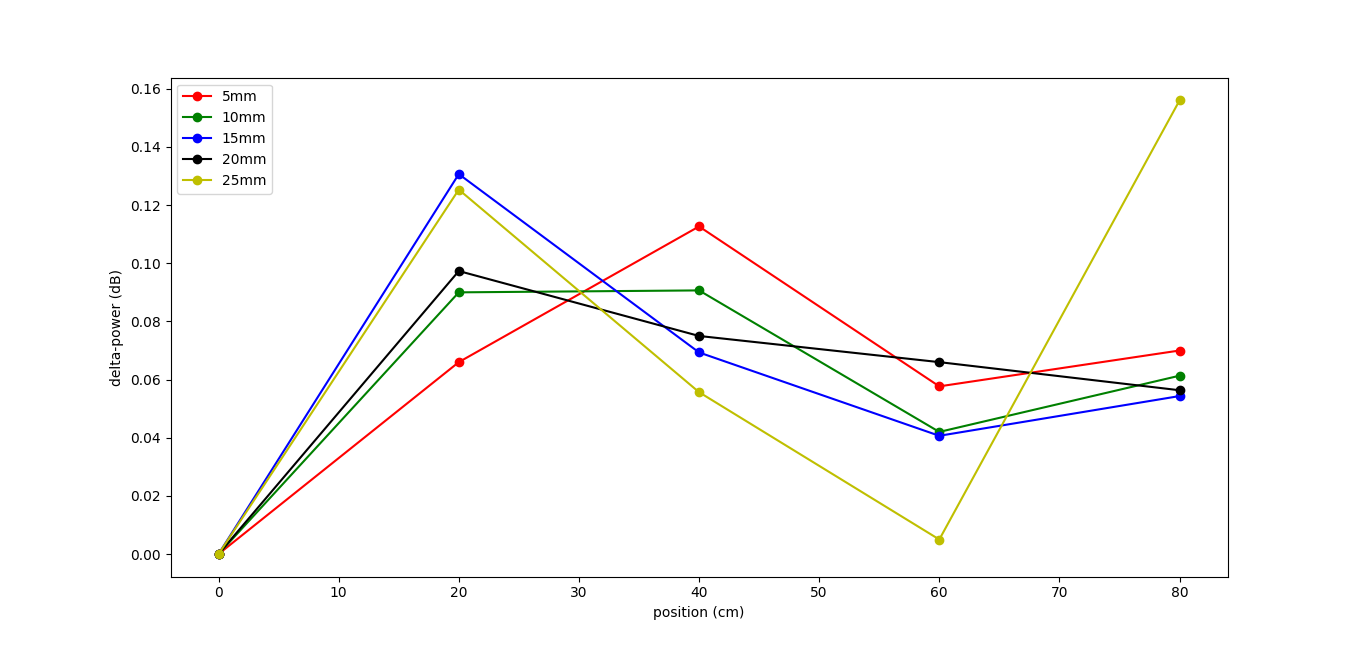
\includegraphics[width=\textwidth]{images/splice_1}
		\caption{}
	\end{subfigure}
	\begin{subfigure}[b]{0.4\textwidth}
		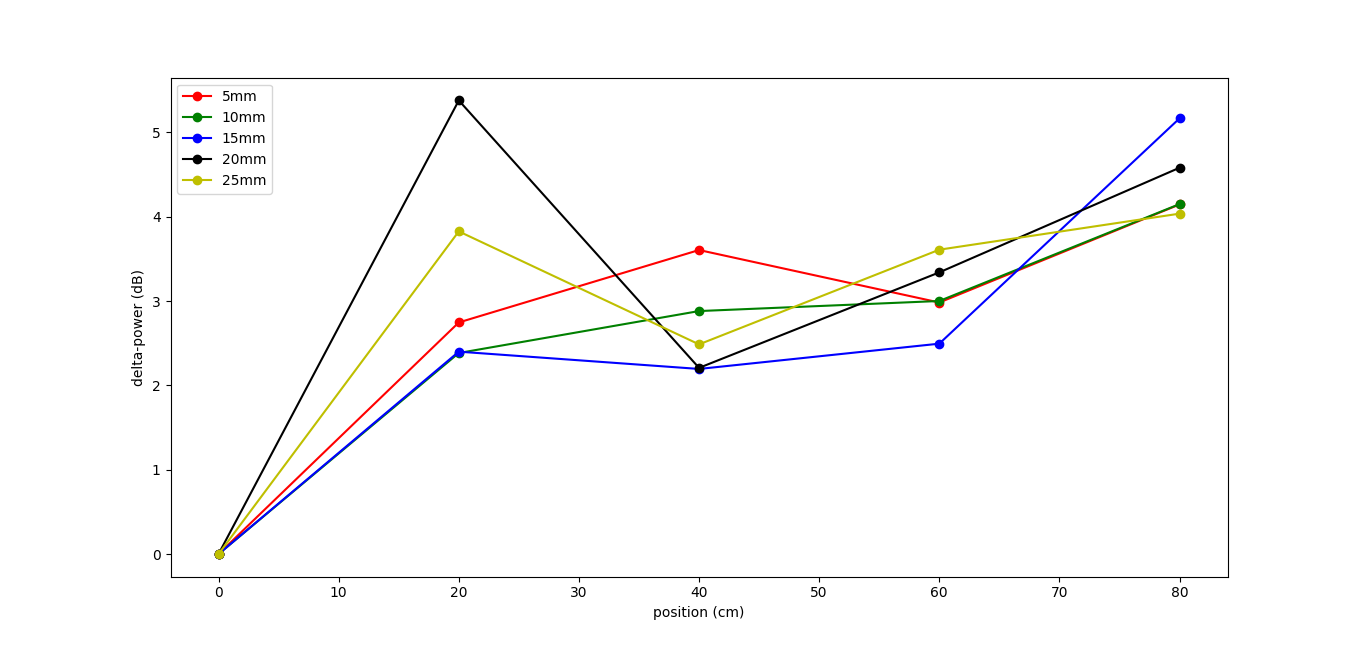
\includegraphics[width=\textwidth]{images/end_1}
		\caption{}
	\end{subfigure}
	\caption[Setup Diagram]{\small{(a) 1m fiber-splice response difference. (b) (a) 1m fiber-end response difference}}
\end{figure}

%=============================================================================
\newpage

\begin{figure}[h!]
	\centering
	\captionsetup{justification=centering}
	\begin{subfigure}[b]{0.4\textwidth}
		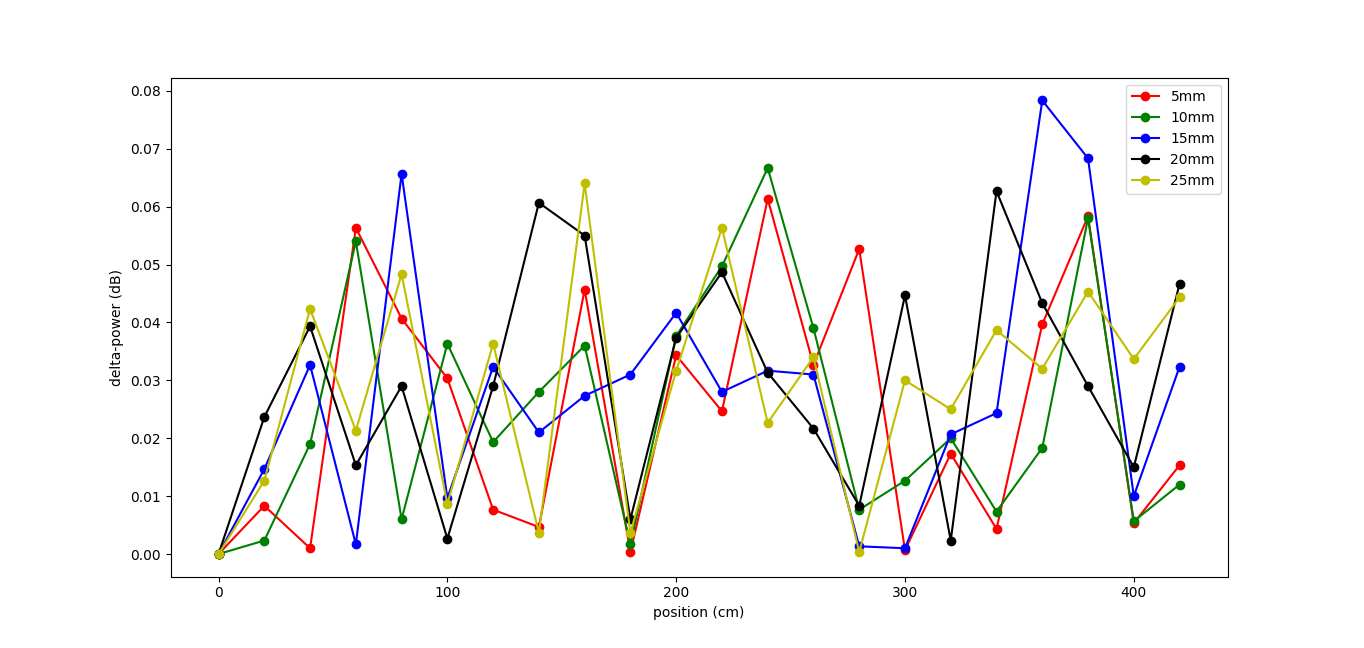
\includegraphics[width=\textwidth]{images/splice1_5}
		\caption{}
	\end{subfigure}
	\begin{subfigure}[b]{0.4\textwidth}
		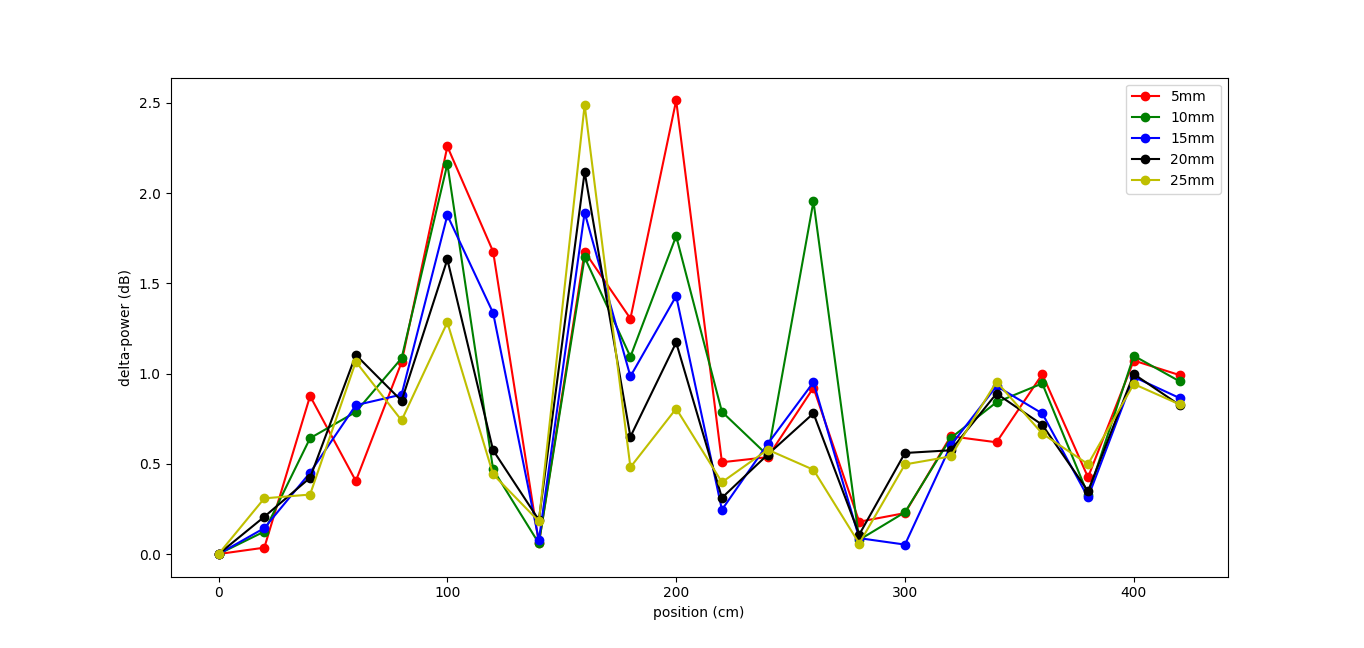
\includegraphics[width=\textwidth]{images/end_5}
		\caption{}
	\end{subfigure}
	\caption[Setup Diagram]{\small{(a) 5m fiber-splice response difference. (b) (a) 5m fiber-end response difference}}
\end{figure}

Another important consideration is about multiple point displacement.
For two point displacement with distance 20mm each other and 10mm displacement value, the only significant result is on single-mode only setup at 1m.
The result show power drop approximately 3dB on first displacement and 0.5dB on second displacement. 

\begin{figure}[h!]
	\centering
	\captionsetup{justification=centering}
	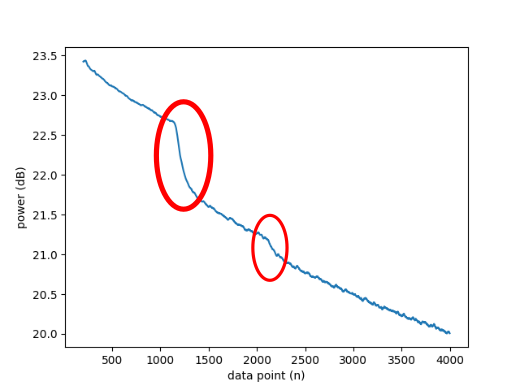
\includegraphics[width=0.4\linewidth]{images/base_2}
	\caption[Setup Diagram]{\small{Trace result on two point displacement}}
\end{figure}
  
  
\bibliographystyle{IEEEtran}
\bibliography{IEEEabrv,/home/achmadi/Documents/BibTex/library.bib}

\end{document}
